\documentclass[a4paper,12pt]{article}
\usepackage[utf8]{inputenc}
\usepackage{amsmath, amssymb}
\usepackage{graphicx}
\usepackage{float}
\usepackage{booktabs}
\usepackage{hyperref}
\usepackage{geometry}
\geometry{margin=2.5cm}

\title{Entrega Práctica 3}
\author{
  Francisco Elías. E-1217/3 \\
  Sebastián Morales. M-6501/3
}
\date{}

\begin{document}

\maketitle
\hrule
\vspace{1em}


\section*{Problema 1}

Al expresar el problema en la forma \( x'(t) = A \cdot x(t) + B \cdot u \), se tiene que la matriz \( A \) es el escalar \( -a \), mientras que \( B \cdot u = 0 \) dado que no hay entradas. Por lo tanto, la solución analítica estará dada por:

\[
\frac{dx}{dt} = -a \cdot x(t)
\]
\[
\frac{1}{x(t)} \, dx = -a \, dt
\]
\[
\int \frac{1}{x(t)} \, dx = \int -a \, dt
\]
\[
\ln(|x(t)|) = -a t + C
\]
\[
|x(t)| = e^{-a t + C} = e^C \cdot e^{-a t}
\]

Sea \( k = e^C \), entonces:

\[
|x(t)| = k \cdot e^{-a t}
\]

Dado que la solución es una función exponencial positiva, se tiene:

\[
x(t) = k \cdot e^{-a t}
\]

Aplicando la condición inicial \( x(0) = x_0 \):

\[
x(0) = k \cdot e^{-a \cdot 0} = x_0
\]
\[
k \cdot e^0 = x_0 \Rightarrow k = x_0
\]

Por lo tanto, la solución es:

\[
x(t) = x_0 \cdot e^{-a t}
\]


En la figura puede apreciarse que la implementación de la solución analítica en Octave resulta en la curvatura exponencial esperada.

\begin{figure}[H]
\centering
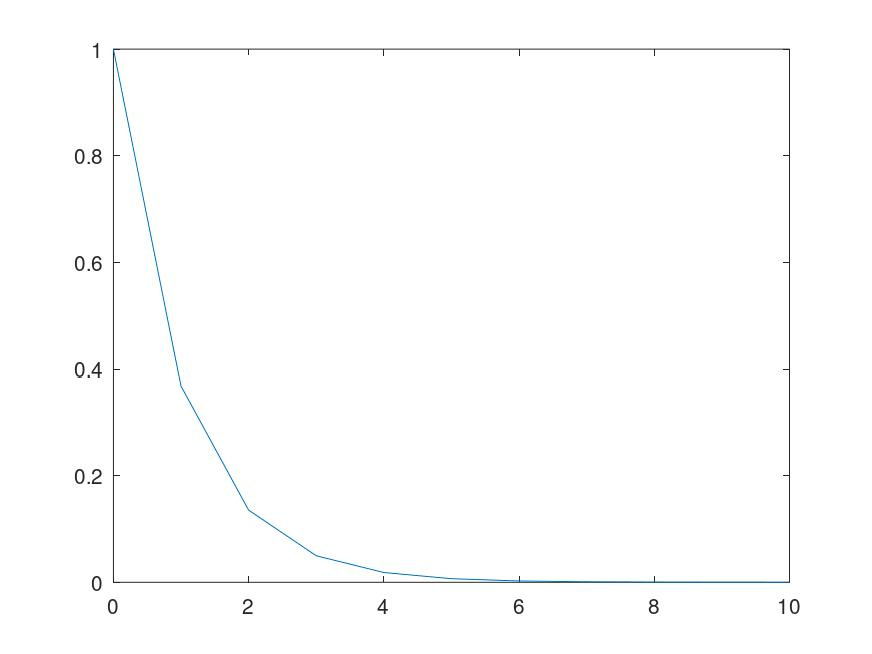
\includegraphics[width=0.75\textwidth]{img/ej1.jpeg}
\caption{Fármaco}
\end{figure}

\section*{Problema 2}

La implementación de \texttt{ltiSolve} emplea la ecuación 2b en cada valor del arreglo de tiempo eficientemente, haciendo uso del método \texttt{expm} para calcular la exponencial matricial necesaria.

\begin{figure}[H]
\centering
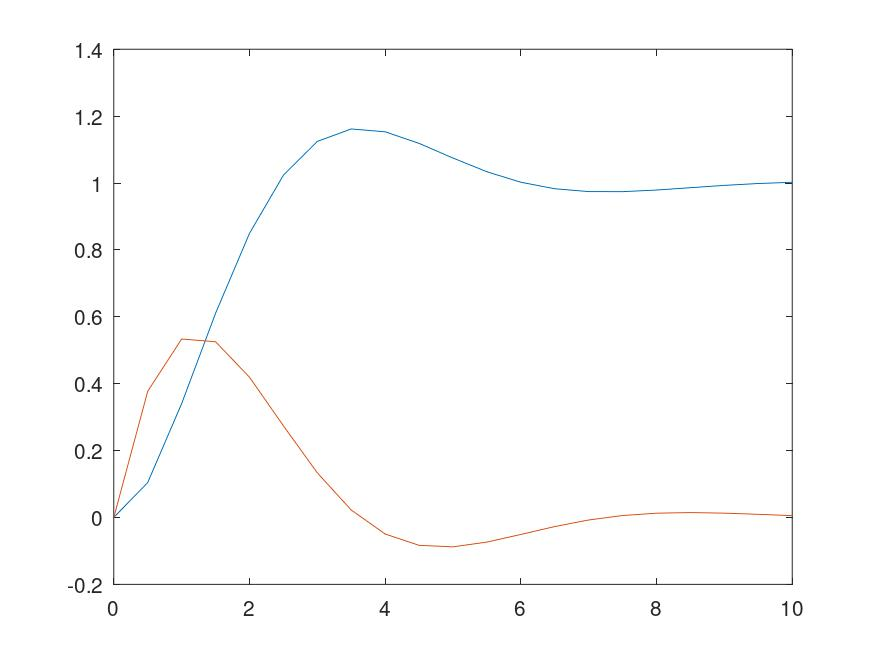
\includegraphics[width=0.75\textwidth]{img/ej2.jpeg}
\caption{ltisolve}
\end{figure}

\section*{Problema 3}

De las ecuaciones de estado pueden obtenerse los siguientes valores para la solución analítica:

\[
A = \begin{bmatrix}
0 & 1 \\
-\frac{k}{m} & -\frac{b}{m}
\end{bmatrix}, \quad
B = \begin{bmatrix}
0 \\
\frac{F}{m}
\end{bmatrix}, \quad
u = 1
\]

El valor inicial \( x_0 \) será:

\[
x_0 = \begin{bmatrix}
0 \\
0
\end{bmatrix}
\]
\subsection*{Con \( b = 1 \):}
\begin{figure}[H]
\centering
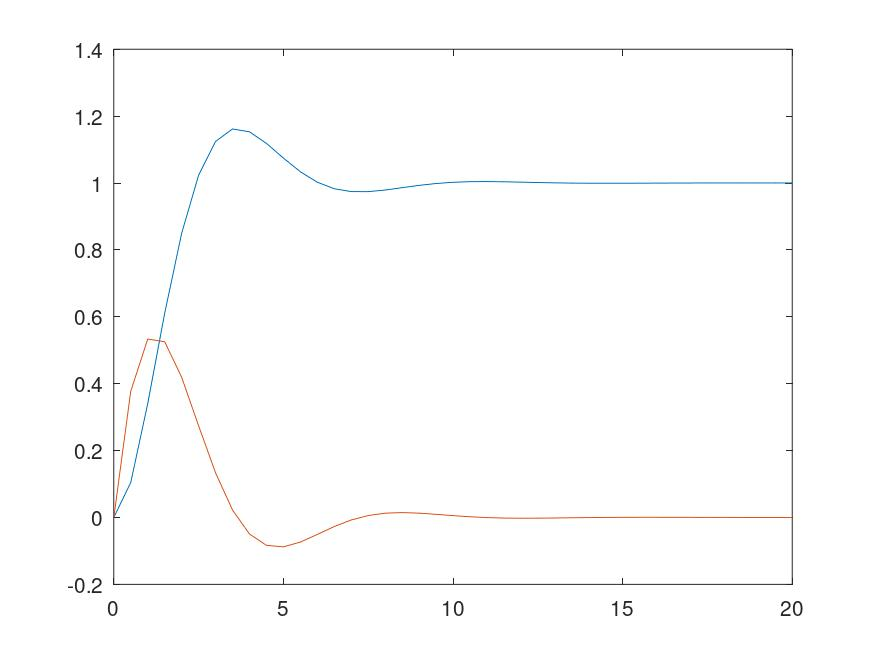
\includegraphics[width=0.75\textwidth]{img/ej3_1.jpeg}
\caption{Resorte con ltisolve, \( b = 1 \)}
\end{figure}

\subsection*{Con \( b = 0 \):}
Oscila indefinidamente debido a que el rozamiento es nulo.

\begin{figure}[H]
\centering
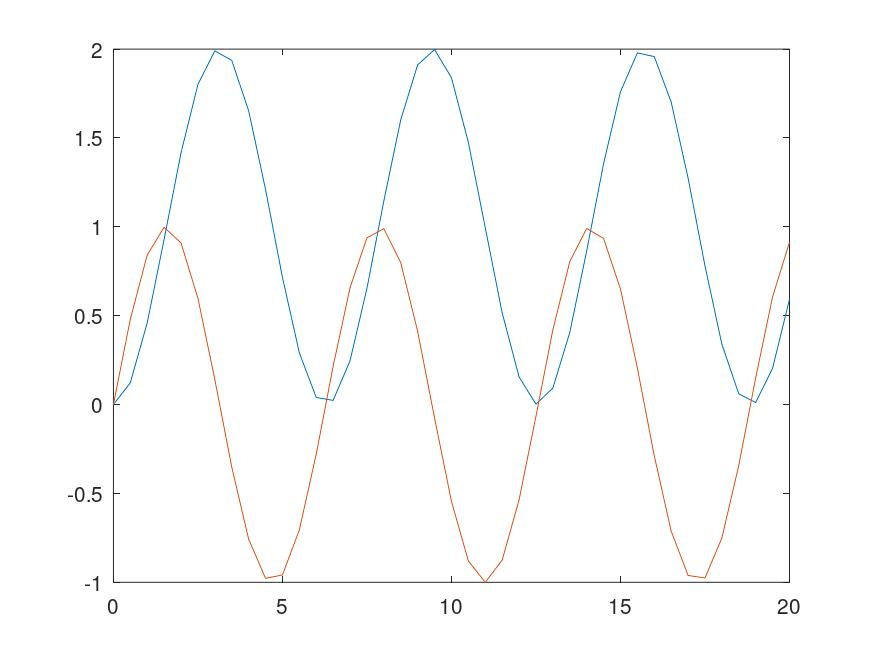
\includegraphics[width=0.75\textwidth]{img/ej3_2.jpeg}
\caption{Resorte con ltisolve, \( b = 0 \)}
\end{figure}

\subsection*{Con \( b = 10 \):}
Movimiento muy lento debido a la elevada fricción con el suelo.

\begin{figure}[H]
\centering
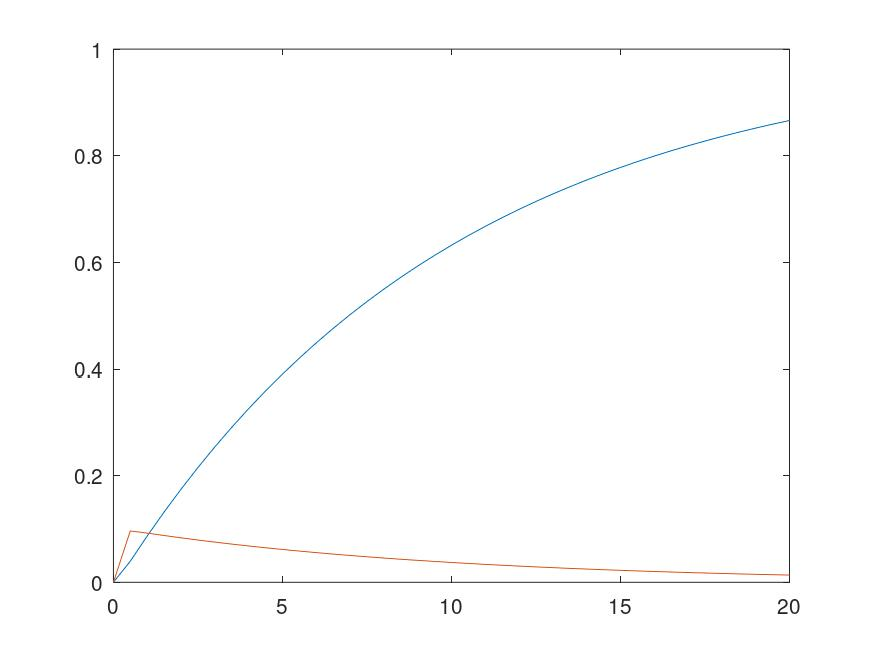
\includegraphics[width=0.75\textwidth]{img/ej3_3.jpeg}
\caption{Resorte con ltisolve, \( b = 10 \)}
\end{figure}

\section*{Problema 4}

Los resultados de las simulaciones hechas con la implementación de Forward Euler tienen una evolución muy similar a las soluciones analíticas vistas anteriormente.

\subsection*{Problema del fármaco:}

\begin{figure}[H]
\centering
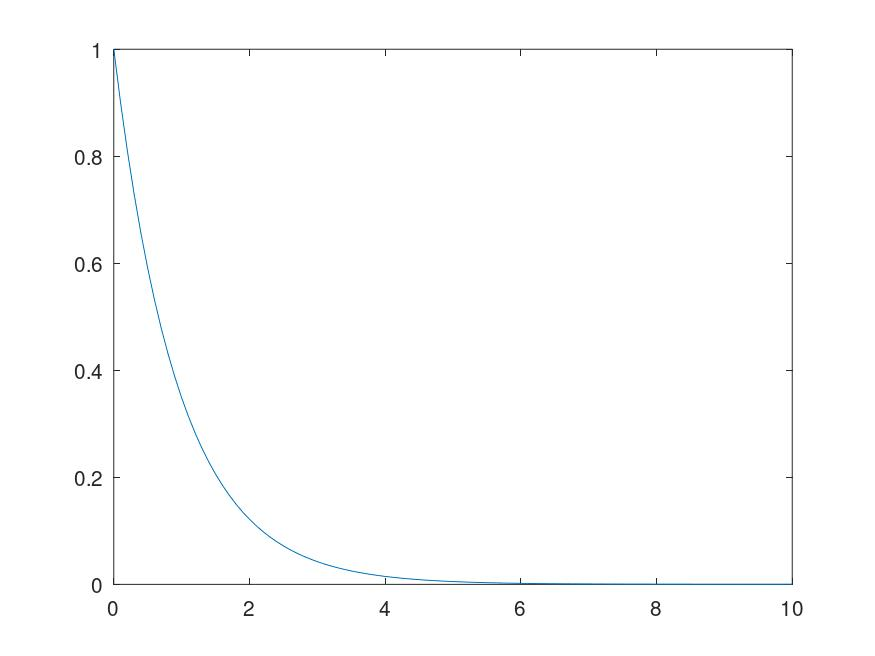
\includegraphics[width=0.75\textwidth]{img/ej4_1.jpeg}
\caption{Fármaco con Forward Euler}
\end{figure}

\subsection*{Problema del resorte:}

\begin{figure}[H]
\centering
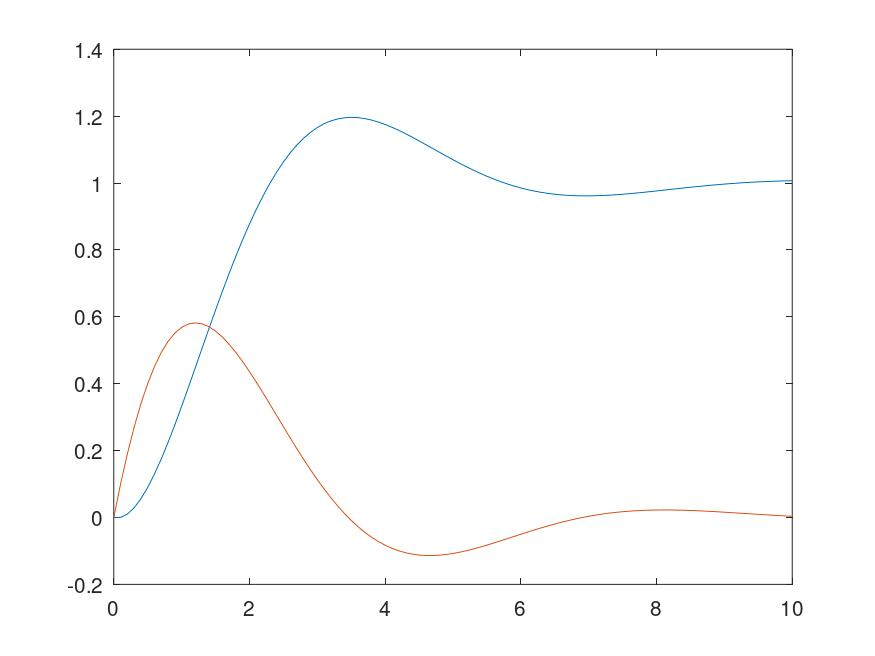
\includegraphics[width=0.75\textwidth]{img/ej4_2.jpeg}
\caption{Resorte con Forward Euler}
\end{figure}


\section*{Problema 5}

Debajo se encuentran los errores obtenidos para las simulaciones con las dos longitudes de paso solicitadas. A partir de los resultados se podría afirmar que Forward Euler es un algoritmo de primer orden, ya que al disminuir 10 veces la longitud de paso se obtiene un error de primer paso \(10^2\) veces menor, pero un error máximo 10 veces menor.

\begin{table}[H]
\centering
\begin{tabular}{@{}ccc@{}}
\toprule
Paso (h) & Error primer paso & Error máximo \\
\midrule
0.1 & 9.8293e-03 & 0.066139 \\
0.01 & 9.9833e-05 & 6.1432e-03 \\
\bottomrule
\end{tabular}
\end{table}

\section*{Problema 6}

Los resultados experimentales para cada coeficiente de roce \( b \) fueron los siguientes:

\begin{itemize}
    \item \( b = 1 \): simulación marginalmente estable con un paso \( h = 1 \). Con valores menores es estable, mientras que con valores mayores se vuelve inestable.
    \item \( b = 0 \): los resultados fueron inestables para todas las longitudes de paso empleadas.
    \item \( b = 10 \): con \( h = 0.1 \) los valores se estabilizan. Con un \( h \) mayor resultan inestables.
\end{itemize}

Para el análisis con autovalores, se hace uso de la función \texttt{eig}:

\begin{verbatim}
- b = 1
A = [0 1; -1 -1]
octave:22> abs(1 + 1 * eig(A))
ans =
   1.0000
   1.0000

- b = 10
A = [0 1; -1 -10]
octave:22> abs(1 + 0.2 * eig(A))
ans =
   0.9798
   0.9798

- b = 0
A = [0 1; -1 0]
octave:41> abs(1 + 0.00001 * eig(A))
ans =
   1.0000
   1.0000
\end{verbatim}

Los resultados obtenidos por prueba y error se acercan bastante a los teóricos máximos. La diferencia fundamental se observa en \( b = 10 \), donde el \( h \) máximo teórico es un poco más de 0.2, a diferencia del 0.1 obtenido experimentalmente. En el caso de \( b = 0 \), aun reduciendo \( h \) a valores ínfimos, los autovalores de \( A_d \) son 1, coincidiendo con lo observado.

\section*{Problema 7}

Para Backward Euler, si bien los errores obtenidos fueron menores que con Forward, no hay una mejora sustancial.

\begin{table}[H]
\centering
\begin{tabular}{@{}ccc@{}}
\toprule
Paso (h) & Error primer paso & Error máximo \\
\midrule
0.1 & 9.0896e-03 & 0.056461 \\
0.01 & 9.9157e-05 & 6.0471e-03 \\
\bottomrule
\end{tabular}
\end{table}

Para el análisis teórico de este método vamos a analizar los autovalores de \( A \) en cada caso para intentar dar una explicación a lo observado, dado que el método presenta estabilidad casi en todos los casos.

\subsection*{b = 1}

Al variar el \( h \), no llegamos a ningún valor en el cual el resultado deje de ser estable.

\begin{verbatim}
A = [0 1; -1 -1]
octave:2> eig(A)
ans =
  -0.5000 + 0.8660i
  -0.5000 - 0.8660i
\end{verbatim}

La parte real de los dos autovalores de \( A \) es menor a 0, por lo que el resultado es siempre estable, coincidiendo con lo observado gráficamente.

\subsection*{b = 10}

\begin{verbatim}
A = [0 1; -1 -10]
octave:4> eig(A)
ans =
  -0.1010
  -9.8990
\end{verbatim}

Nuevamente, la parte real de los autovalores es negativa, lo que garantiza estabilidad.

\subsection*{b = 0}

\begin{verbatim}
A = [0 1; -1 0]
octave:6> eig(A)
ans =
   0 + 1i
   0 - 1i
\end{verbatim}

La parte real de los autovalores es cero, por lo que el sistema es marginalmente estable, pero Backward Euler no puede asegurar estabilidad numérica en este caso, tal como se observó experimentalmente.


\section*{Problema 8}

Para Heun sí se nota una mejora sustancial en la precisión respecto a los dos métodos de Euler anteriormente vistos. Se comprueba que es un método de segundo orden, ya que el error del primer paso disminuye tres órdenes de magnitud y el máximo en dos órdenes al disminuir diez veces la longitud de paso \( h \).

\begin{table}[H]
\centering
\begin{tabular}{@{}ccc@{}}
\toprule
Paso (h) & Error primer paso & Error máximo \\
\midrule
0.1 & 1.7067e-04 & 2.4063e-03 \\
0.01 & 1.6708e-07 & 2.3020e-05 \\
\bottomrule
\end{tabular}
\end{table}

\subsection*{b = 1}
Observamos que \( h \) puede estar oscilando entre 1.4 y 1.5.

\begin{verbatim}
A = [0 1; -1 -1]
octave:61> abs(eig( eye(2,2)+2*A+0.5*(2*A)^2 ))
ans =
   1
   1
\end{verbatim}

Sin embargo, el análisis teórico nos permite estirar un poco más, hasta un paso de 2.

\subsection*{b = 10}
Estimamos que el valor máximo de \( h \) es 0.1 en este caso.

\begin{verbatim}
A = [0 1; -1 -10]
octave:80> abs(eig( eye(2,2)+0.202*A+0.5*(0.202*A)^2 ))
ans =
   0.9798
   0.9996
\end{verbatim}

Teóricamente puede usarse un valor mayor, cercano a 0.202.

\subsection*{b = 0}
El valor máximo de \( h \) observado está entre 0.1 y 0.2.

\begin{verbatim}
A = [0 1; -1 0]
octave:89> abs(eig( eye(2,2)+0.1*A+0.5*(0.1*A)^2 ))
ans =
   1.0000
   1.0000
\end{verbatim}

Según el análisis teórico, el valor máximo es 0.1.

\section*{Problema 9}

Los errores obtenidos con la regla trapezoidal son del mismo orden de magnitud que los obtenidos con Heun, lo cual es esperable para otro método de segundo orden.

\begin{table}[H]
\centering
\begin{tabular}{@{}ccc@{}}
\toprule
Paso (h) & Error primer paso & Error máximo \\
\midrule
0.1 & 9.0615e-05 & 1.1439e-03 \\
0.01 & 8.4156e-08 & 1.1451e-05 \\
\bottomrule
\end{tabular}
\end{table}

La regla trapezoidal mantiene la estabilidad ya que su solución analítica es estable.

\subsection*{b = 1}
Valor máximo de \( h = 2 \):

\begin{verbatim}
A = [0 1; -1 -1]
octave:29> abs(eig( inv(eye(2)-0.5*2*A)*(eye(2)+0.5*2*A) ))
ans =
   0.5774
   0.5774
\end{verbatim}

Teóricamente pueden usarse valores aún mayores.

\subsection*{b = 10}
Sin límite práctico visible de \( h \) que provoque inestabilidad.

\begin{verbatim}
A = [0 1; -1 -10]
octave:34> abs(eig( inv(eye(2)-0.5*2123*A)*(eye(2)+0.5*2123*A) ))
ans =
   0.9815
   0.9998
\end{verbatim}

\subsection*{b = 0}
Valor máximo de \( h \) observado entre 0.1 y 0.2.

\begin{verbatim}
A = [0 1; -1 0]
\end{verbatim}

En este caso, el sistema es marginalmente estable. La regla trapezoidal es un método F-estable que preserva dicha característica, por lo que los autovalores de \( A_d \) serán siempre de módulo 1.

\section*{Problema 10}

Como se vio previamente, el método de Heun se vuelve inestable con pasos \( h \) grandes en el sistema masa-resorte con \( b = 1 \). Es esperable que el paso oscile entre 2 y 4 para mantener el error dentro de los valores admitidos.


\begin{figure}[H]
\centering
\begin{minipage}[b]{0.49\textwidth}
    \centering
    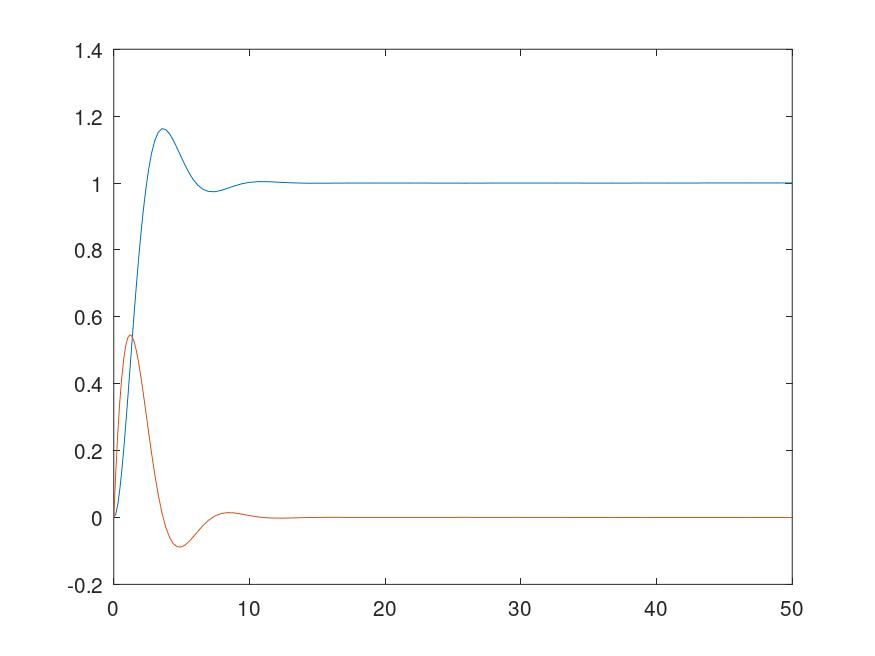
\includegraphics[width=\textwidth]{img/ej10_1.jpeg}
\end{minipage}
\hfill
\begin{minipage}[b]{0.49\textwidth}
    \centering
    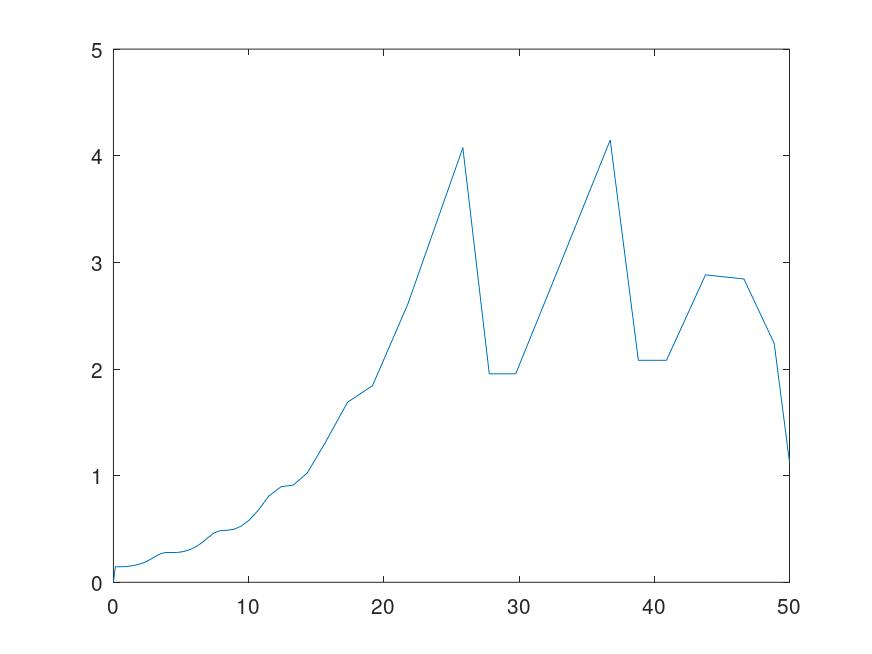
\includegraphics[width=\textwidth]{img/ej10_2.jpeg}
\end{minipage}
\caption{RK23 con \( b = 1 \)}
\end{figure}

\subsection*{b = 100}

La estabilidad solo puede mantenerse con valores muy pequeños de paso, entre 0.02 y 0.04.


\begin{figure}[H]
\centering
\begin{minipage}[b]{0.49\textwidth}
    \centering
    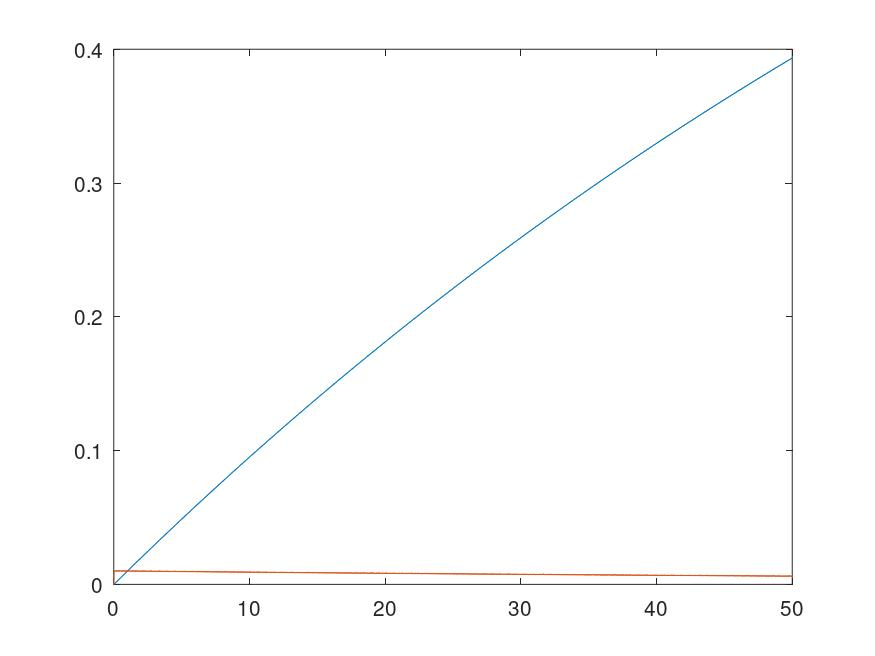
\includegraphics[width=\textwidth]{img/ej10_3.jpeg}
\end{minipage}
\hfill
\begin{minipage}[b]{0.49\textwidth}
    \centering
    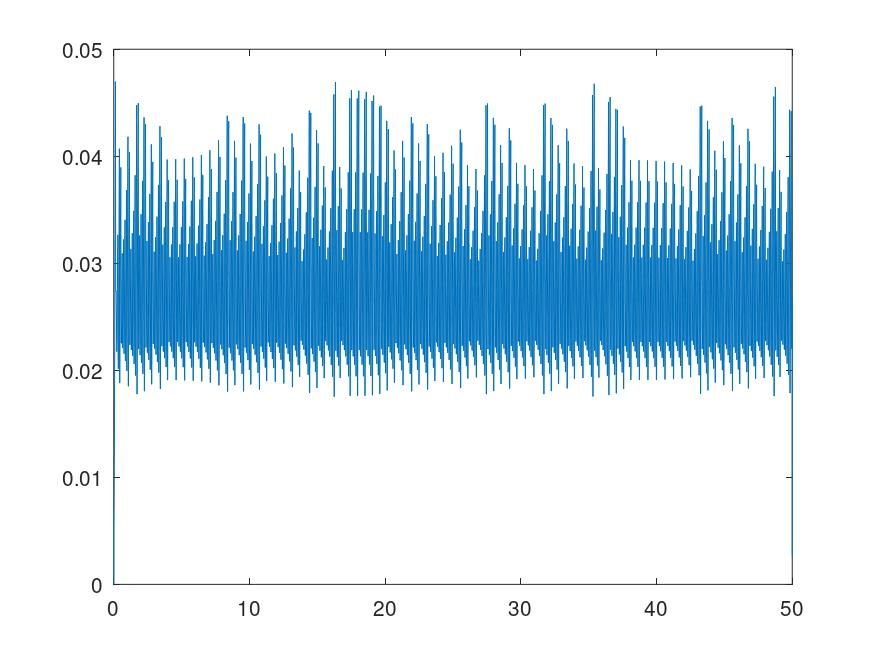
\includegraphics[width=\textwidth]{img/ej10_4.jpeg}
\end{minipage}
\caption{RK23 con \( b = 100 \)}
\end{figure}

\section*{Problema 11}

A diferencia del caso anterior, el uso de un método implícito permite preservar la estabilidad numérica del sistema original. Las simulaciones con \( b = 1 \) y \( b = 100 \) no presentan errores grandes y permiten usar pasos considerablemente mayores que los logrados con RK23.


\begin{figure}[H]
\centering

\begin{minipage}[b]{0.48\textwidth}
    \centering
    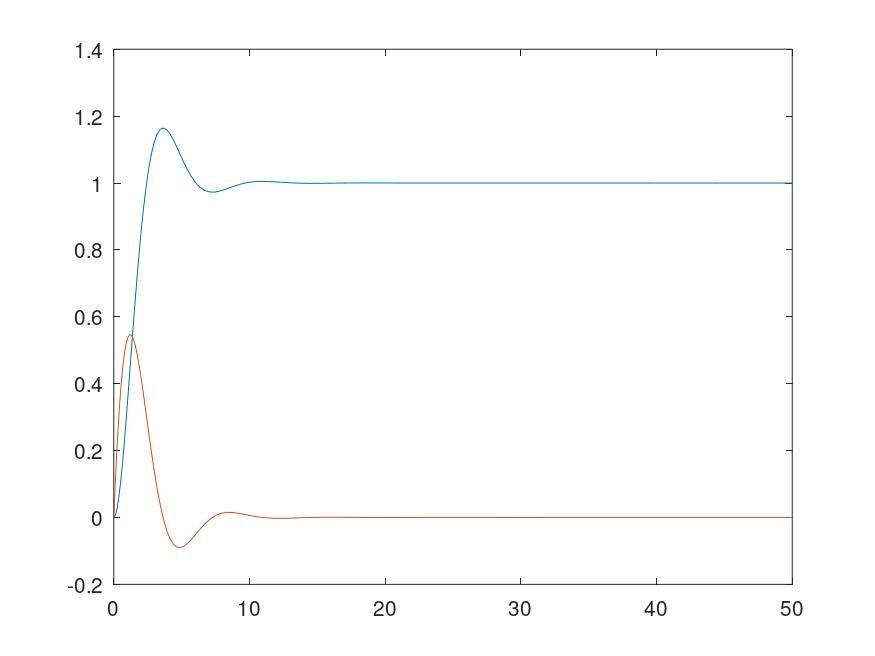
\includegraphics[width=\textwidth]{img/ej11_1.jpeg}
\end{minipage}
\hfill
\begin{minipage}[b]{0.48\textwidth}
    \centering
    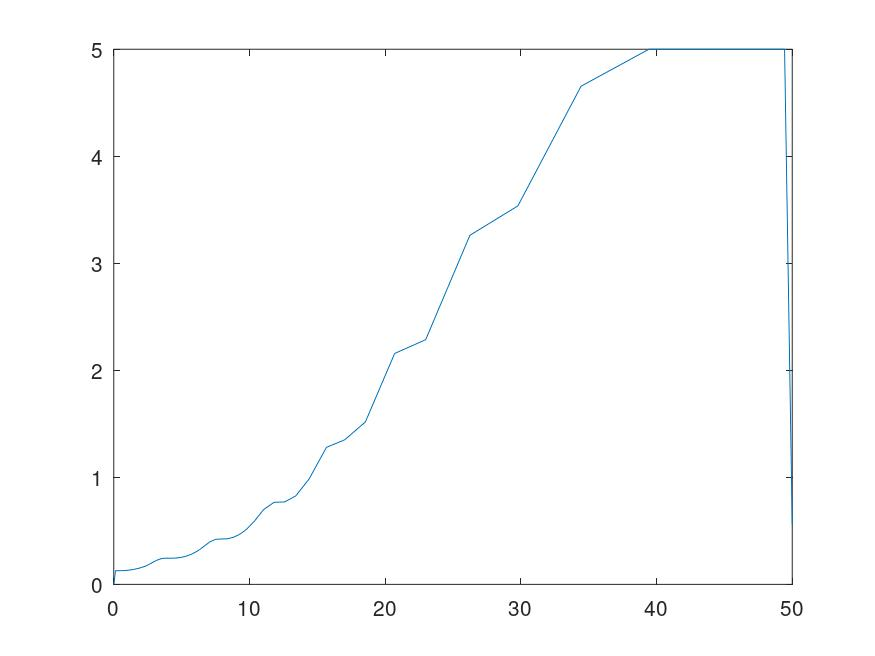
\includegraphics[width=\textwidth]{img/ej11_2.jpeg}
\end{minipage}

\vspace{0.5em}

\begin{minipage}[b]{0.48\textwidth}
    \centering
    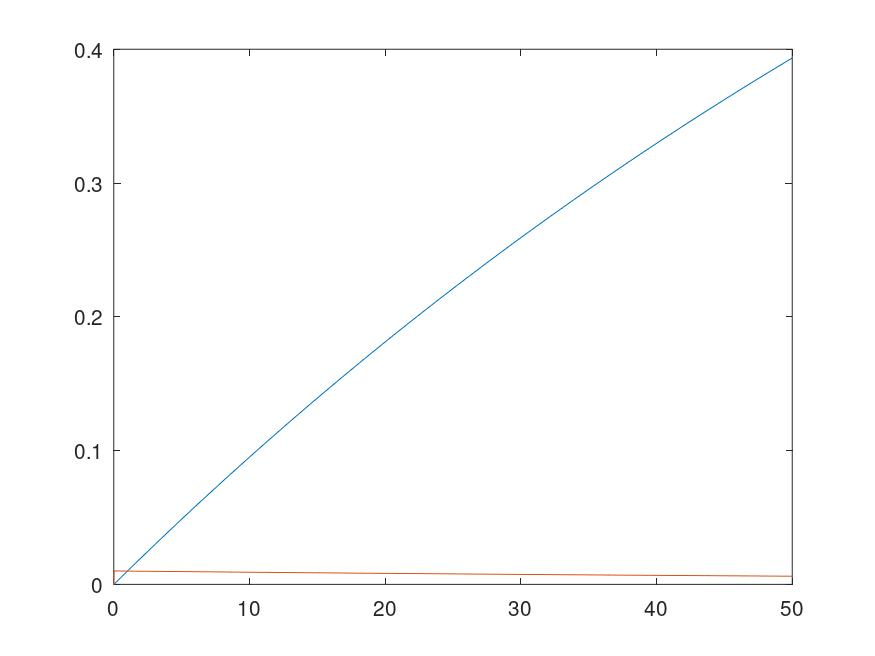
\includegraphics[width=\textwidth]{img/ej11_3.jpeg}
\end{minipage}
\hfill
\begin{minipage}[b]{0.48\textwidth}
    \centering
    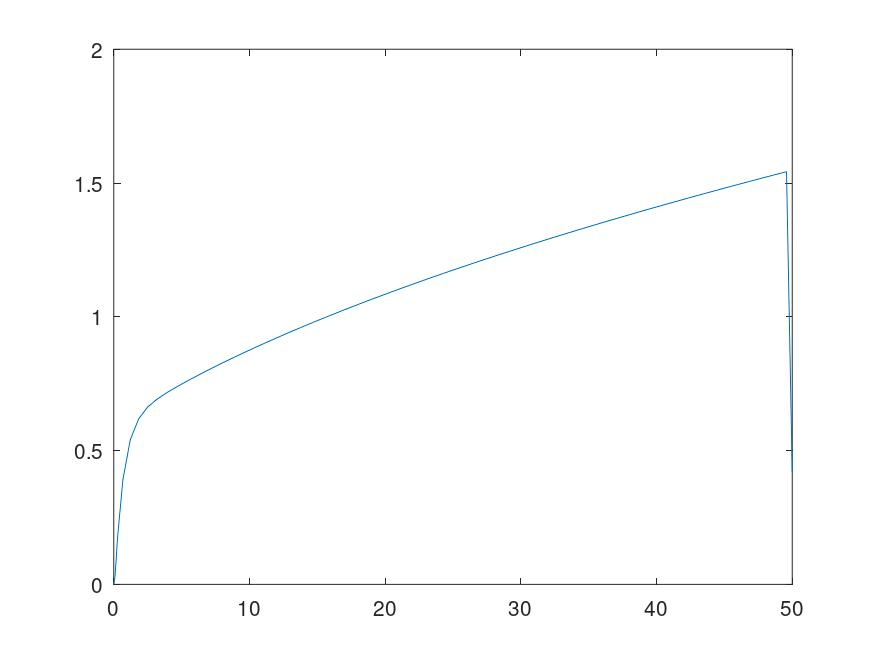
\includegraphics[width=\textwidth]{img/ej11_4.jpeg}
\end{minipage}

\caption{Método implícito con \( b = 1 \) (arriba) y \( b = 100 \) (abajo).}
\end{figure}

\subsection*{b = 0}

Dado que se busca preservar la estabilidad marginal, es necesario usar un tamaño de paso pequeño debido a la alta frecuencia de oscilación. Como los valores se modifican con rapidez, pasos grandes deforman las soluciones y aumentan el error.

\begin{figure}[H]
\centering
\begin{minipage}[b]{0.49\textwidth}
    \centering
    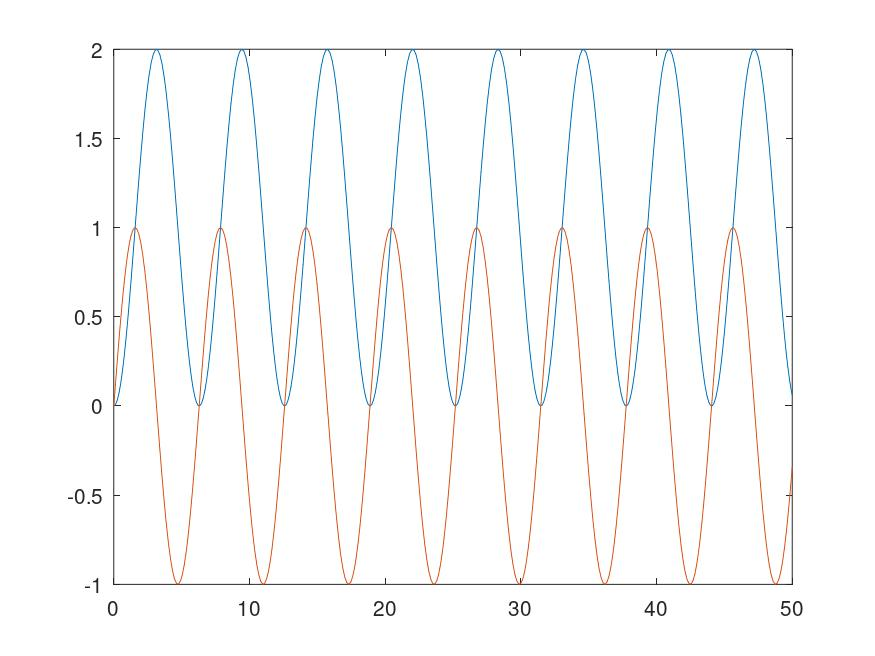
\includegraphics[width=\textwidth]{img/ej11_5.jpeg}
\end{minipage}
\hfill
\begin{minipage}[b]{0.49\textwidth}
    \centering
    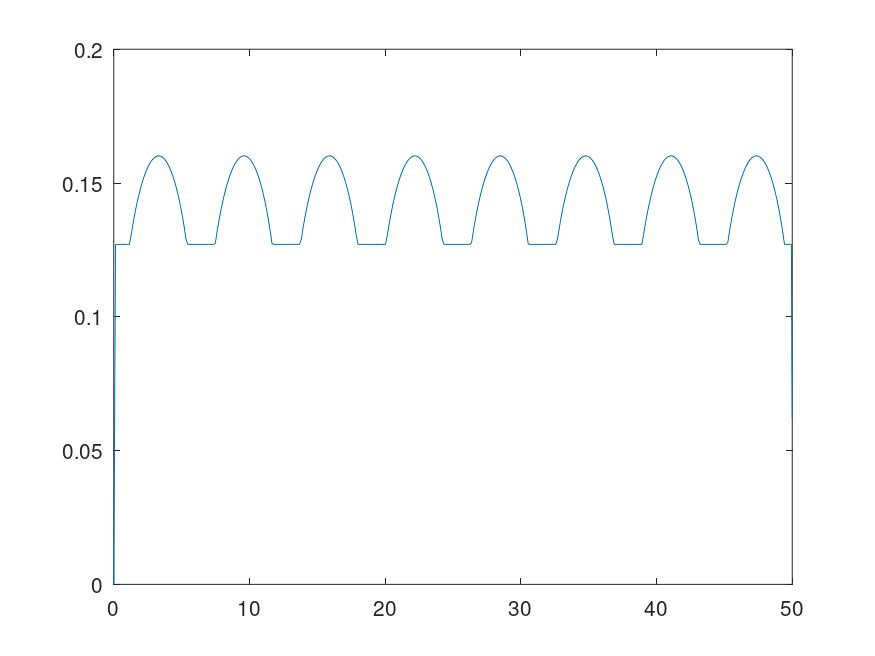
\includegraphics[width=\textwidth]{img/ej11_6.jpeg}
\end{minipage}
\caption{Método implícito con \( b = 0 \)}
\end{figure}

\end{document}
